
\subsection{Punto \textbf{2a}}

\begin{itemize}
\item \emph{\textbf{Simular el inversor con el programa HSPICE y comparar con los resultados del punto anterior. Utilizar una señal de entrada con $t_{rise} = t_{fall} = 1 \si[per-mode=symbol]{\pico\second}$. Incluir en el informe una captura de pantalla que muestre la configuración de los parámetros de cada MOSFET.}}
\end{itemize}

Para este punto se dibujó el circuto correspondiente en el editor de esquemáticos del programa synopsys en una nueva biblioteca creada para los circuitos y layouts que se crearon. En la figura~\figref{fig:fig_inverter_schematic} puede verse el circuito diseñado, y pueden verse los parámetros seleccionados para los transistores.




\begin{figure}[H] %htb
\begin{center}
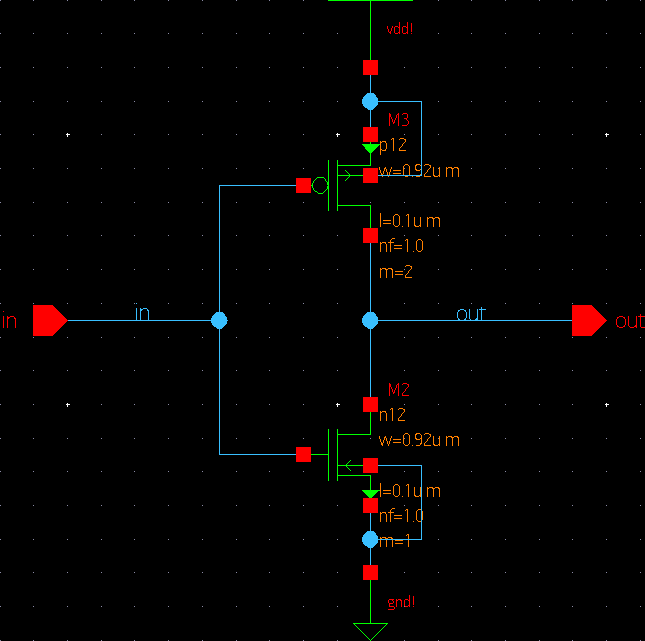
\includegraphics[width=0.85 \textwidth, angle=0]{./img/point2/TEST_LOGIC_GATES_Inverter_schematic}
\caption{\label{fig:fig_inverter_schematic}\footnotesize{Inversor \textbf{CMOS} diseñado (esquemático).}}
\end{center}
\end{figure}


En la figura~\figref{fig:fig_inverter_same_load_schematic} puede verse el circuito del test bench armado para simular la respuesta del inversor.


\begin{figure}[H] %htb
\begin{center}
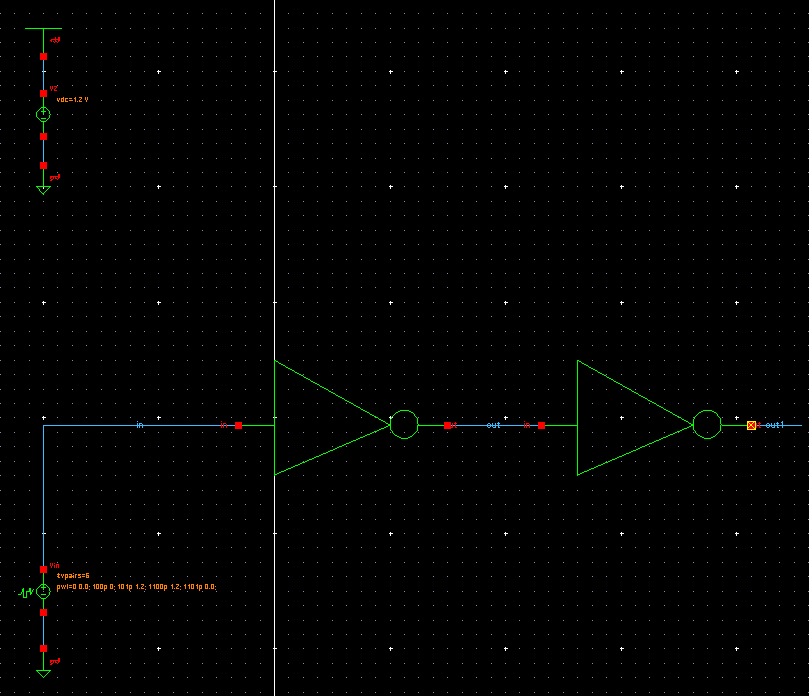
\includegraphics[width=0.85 \textwidth, angle=0]{./img/point2/TEST_LOGIC_GATES_tb_inverter_same_load_schematic}
\caption{\label{fig:fig_inverter_same_load_schematic}\footnotesize{Inversor \textbf{CMOS} cargado con inversor idéntico, test bench diseñado (esquemático).}}
\end{center}
\end{figure}


En la figura~\figref{fig:fig_inverter_same_load_response} puede verse la respuesta obtenida con el circuito de prueba de la figura~\figref{fig:fig_inverter_same_load_schematic}. El valor de tiempo de retardo obtenido para esta respuesta es de:


\begin{equation*}
\mathcolorbox{Cyan}{ T_{delay} = 7.4514 \si[per-mode=symbol]{\pico\second} }
\end{equation*}

Que está en el orden de lo hallado por cálculo en la sección~\sectref{calculated_val}, pero es bastante disímil.


\vfill


\clearpage



\begin{figure}[H] %htb
\begin{center}
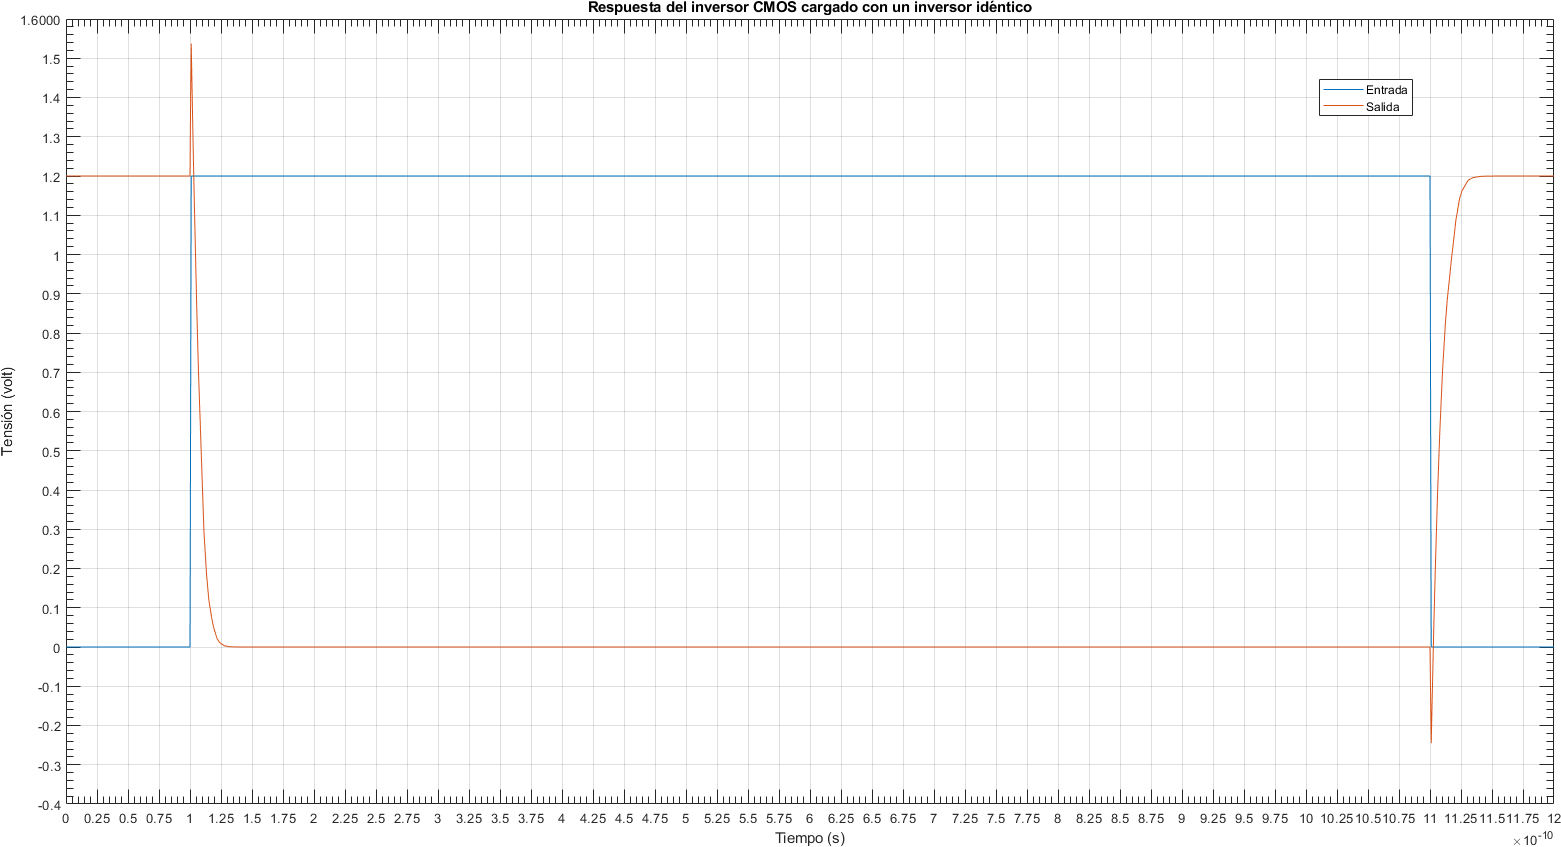
\includegraphics[width=0.92 \textheight, angle=90]{./img/point2/same_load_response}
\caption{\label{fig:fig_inverter_same_load_response}\footnotesize{Respuesta del inversor \textbf{CMOS} cargado con inversor idéntico.}}
\end{center}
\end{figure}


\clearpage